



\section{Stress and the autonomic nervous system}

% This chapter examines the individual components of this reasearch. It starts with a deeper look at stress and its impact on the Autonomic Nervous System, followed by a discussion on heart rate and heart rate variability. Moreover, the concept of rPPG, the mechanism of biofeedback, and the influence of music on stress regulations are investigated.

This chapter starts with a deeper look  at stress and its impact on the autonomic nervous system. It explains why stress has an impact on the cardiovascular system. Moreover, it differentiates between the heart rate and the heart rate variability.

The autonomic nervous system consists of the parasympathetic and the sympathetic branches. The parasympathetic system acts during periods of rest and calm and regulates functions such as rest and digest. In contrast, the sympathetic system is activated in situations in which we perceive a threat. In these cases, the heart rate increases to release more energy \cite{mccorry2007physiology}.

McEwen (2007) describes this as the allostatic effect. The body dynamically adjusts its internal state to meet the standards of the environment. For instance, in a life threatening situation a lot of energy is released. The short-term mobilization of energy is a protective reaction of the body. If this activation occurs chronically without enough recovery, it can lead to permenant damage (Figure \ref{fig:allostatic_load}) \cite{mcewen2017neurobiology}.

Individual differences in stress perception are rooted in the brain's ability to evaluate environmental stimuli. According to McEwen (2007), the brain exhibits significant plasticity, meaning its responses to stressors are shaped by genetics, early development, and past experiences. If an individual has for example experienced a trauma, the brain’s system may become hypersensitive \cite{mcewen2017neurobiology}. It might trigger a ‘fight or flight’ response in harmless situations\cite{mccorry2007physiology}. This can lead to coping strategies, such as smoking or drinking. These coping strategies try to calm down the sympathetic branch of the autonomic nervous system. On the other hand, the plasticity also allows for an intervention in the other direction. The brain can be trained to shift from a threatening state to a calm state \cite{mcewen2017neurobiology}.

\begin{figure}[!ht]
    \centering
    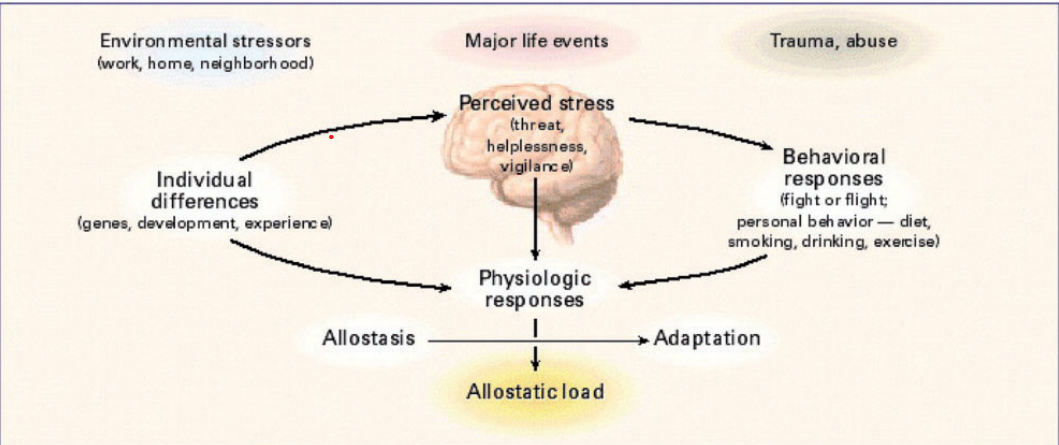
\includegraphics[width=0.9\columnwidth]{./chapters/pictures/test.png}
    \caption{The figure illustrates the mechanism of allostatic load and the underlying pathways of stress perception and physiological adaptation \cite{mcewen2017neurobiology}.}
    \label{fig:allostatic_load}
\end{figure}


When monitoring the heart, it is crucial to differentiate between the heart rate and the heart rate variability. The heart rate can be thought of as the quantity and the heart rate variability as the quality of heart activity\cite{shaffer2017overview}.

The heart rate measures the total number of heartbeats per minute. It reflects how fast the heart is beating at any given moment. However, it can be described as a relatively coarse metric. Therefore, it is a releative insensitive marker for early-stage stress \cite{shaffer2017overview}.

Heart Rate Variability (HRV), on the other hand, focuses on the smaller level of cardiac timing. It describes  the fluctuation in the time intervals between two heartbeats. This is defined as Interbeat Intervals (IBIs). HRV consists of the constant changes in these time intervals from one beat to the next \cite{shaffer2017overview}.

From a physiological standpoint, a healthy biological system needs to be highly adaptable. This means that a healthy heart does not maintain a perfectly rigid or identical time between intervals. Instead, the autonomic nervous system constantly changes the timing of each beat to respond to internal and external demands \cite{shaffer2017overview}.

If the intervals between heartbeats become too consistent and lose this natural irregularity, it is often a clinical sign of physiological strain or a lack of regulatory flexibility. High variability indicates that the body is in a state of balance and can rapidly adjust to stressors. Therefore, while HR measures the quantity of beats, HRV reflects the quality and efficiency of the autonomic nervous system’s control over the cardiovascular system \cite{shaffer2017overview}.









